%!TEX program = lualatex
\documentclass[12pt,letterpaper,twoside]{article}
%!TEX root = ./set_cover_problem.tex

% Pro­gram­ming fa­cil­i­ties
	\usepackage{etoolbox}
	\usepackage{ifxetex}
	\usepackage{ifluatex}

% Encoding
	\usepackage[T1]{fontenc}
	\ifboolexpr{bool{xetex} or bool{luatex}}{%
		\usepackage{fontspec}
	}{%
		\usepackage[utf8]{inputenc}
	}

% Language
	\usepackage[english,french]{babel} % Second language = main language

% Show a summary of the layout of the current document with \layout.
	%\usepackage{layout}

% For easy management of document margins and the document page size.
	\usepackage[top=2cm, bottom=1.8cm, left=1.8cm, right=1.8cm, head=14pt, foot=36pt]{geometry}

% Lets you change line spacing.
	%\usepackage{setspace}

% Euro symbol
	%\usepackage{eurosym}

% Fonts (include only one)
	%\usepackage{bookman}
	%\usepackage{charter}
	%\usepackage{newcent}
	\usepackage{lmodern}
	%\usepackage{mathpazo}
	%\usepackage{mathptmx}

% Enables typesetting of hyperlinks
	%\usepackage{url}
	\usepackage{hyperref}

% Verbatim environment
	%\usepackage{verbatim}
	%\usepackage{moreverb}
	\usepackage{fancyvrb}

% Code listing
	\usepackage{listings}

% To change header and footer of any page of the document.
	\usepackage{fancyhdr}

% Allows you to insert graphic files within a document.
	%\usepackage{graphicx}

% Allows figures or tables to have text wrapped around them.
	%\usepackage{wrapfig}

% Adds support for colored text.
	\usepackage{xcolor}

% Allows tables rows and columns to be colored, and even individual cells.
	%\usepackage{colortbl}

% Mathematics
	\usepackage{amsmath}
	\usepackage{amssymb}
	\usepackage{mathrsfs}
	\usepackage{amsthm}
	\usepackage{dsfont}
	\usepackage{braket}
	\usepackage{stmaryrd}
	%\usepackage{mathtools}
	%\usepackage{bm} % Greek letters in math mode

% Tables
	\usepackage{array}
	\usepackage{tabularx}
	\usepackage{multirow}
	\usepackage{booktabs}

% Provides control over the layout of the three basic list environments: enumerate, itemize and description.
	%\usepackage{enumitem}

% Interface to sectioning commands for selection from various title styles
	\usepackage[nobottomtitles]{titlesec}

% Highly customized stacking of objects, insets, baseline changes, etc.
	\usepackage{stackengine}

% Routines for constrained scaling and stretching of objects, relative to a reference object or in absolute terms
	\usepackage{scalerel}

% \rel­size command
	\usepackage{relsize}

% Provides control over the typography of the Table of Contents, List of Figures and List of Tables, and the ability to create new ‘List of ...’.
	\usepackage{tocloft}
	\usepackage{titletoc}

% Advanced bibliography handling.
	%\usepackage{bibtex}
	\usepackage[backend=bibtex,bibstyle=ieee,citestyle=numeric-comp]{biblatex}

% Allows customization of appearance and placement of captions for figures, tables, etc.
	\usepackage[justification=centering]{caption}

% Provides the multicols environment which typesets text into multiple columns.
	%\usepackage{multicol}

% This package simplifies the insertion of external multi-page PDF or PS documents.
	%\usepackage{pdfpages}

% Prints out all index entries in the left margin of the text.
	%\usepackage{showidx}

% Allow to define multiple floats (figures, tables) within one environment giving individual captions and labels in the form 1a, 1b.
	%\usepackage{subcaption}

% Allow TeX pictures or other TeX code to be compiled standalone or as part of a main document
	%\usepackage[subpreambles=true]{standalone}
	\usepackage[mode=tex]{standalone}
	\usepackage{import}

% Floating elements placement
	\usepackage{float}

% PGF-TikZ
	\usepackage{pgf}
	\usepackage{pgfplots}
	\pgfplotsset{compat=1.16}
	\usepackage{tikz}
	\usepackage{tikzpeople}

% Lets you insert notes of stuff to do with the syntax \todo{Add details.}.
	%\usepackage{todonotes}

% Text Companion fonts, which provide many text symbols (such as baht, bullet, copyright, musicalnote, onequarter, section, and yen), in the TS1 encoding.
	\usepackage{textcomp}

% Add document elements like a bibliography or an index to the Table of Contents.
	\usepackage[notindex,nottoc,notlot,notlof]{tocbibind}

%!TEX root = ./PARL.tex

%=======================================================================================================
%=============================================== Informations ==========================================
%=======================================================================================================

% Cover infos
\title{Rapport intermédiaire: problème de couverture d'ensemble}
\author{Benoît Cortier \& Maxime Pinard}
\date{\today{}}

% Fancy style options
\lhead{\small Benoît Cortier \& Maxime Pinard}
\rhead{\small Couverture d'ensemble}
\chead{}
\lfoot{}
\rfoot{}
\cfoot{\thepage}
\pagestyle{fancy}

%% Redefine the fancy plain page style
%\fancypagestyle{plain}{
%	\fancyhf{}
%	\lhead{\small Benoît Cortier \& Maxime Pinard}
%	\rhead{\small PARL}
%	\chead{}
%	\lfoot{}
%	\rfoot{}
%	\cfoot{\thepage}
%}

%=======================================================================================================
%================================================== Configs ============================================
%=======================================================================================================

% Figures folder
\graphicspath{{figures/}}

% Prevent page breaks in paragraphs
\predisplaypenalty=1000
\postdisplaypenalty=1000
\clubpenalty=1000

% Minimal space required in the bottom margin not to move the title on the next page
\renewcommand{\bottomtitlespace}{.1\textheight}

% Links config, especialy for the table of contents
\hypersetup{
    colorlinks=true,
    linkcolor=black,
    urlcolor=blue,
    linktoc=all
}

% French language config
\frenchbsetup{StandardLayout=true,ReduceListSpacing=false,CompactItemize=false}

% Environments
\theoremstyle{definition}
\newtheorem{thm}{Théorème}
\newtheorem{defn}{Définition}
\newtheorem{prop}{Proposition}

%=======================================================================================================
%================================================= Functions ===========================================
%=======================================================================================================

% Clear to the next left page
\newcommand*{\cleartoleftpage}{
  \clearpage \ifodd\value{page}\hbox{}\newpage\fi
}

% Paragraph with line break
\newcommand{\p}[1]{\paragraph{#1\\}}

% Function to print a warning sign
\newcommand{\dangersign}[1][2.5ex]
	{\renewcommand{\stacktype}{L}
		{\scaleto{\stackon[1pt]{\color{red}$\triangle$}{\fontsize{4pt}{4pt}\selectfont !}}{#1}}}

% Definition of some dt/dx/dy shortcuts for integrals
\newcommand{\dt}
{\;\mathrm{d}\,t}

\newcommand{\dx}
{\;\mathrm{d}\,x}

\newcommand{\dy}
{\;\mathrm{d}\,y}

% Definition of \Witem for 'itemize' environment with a warning sign
\newcommand{\Witem}
{\item[\dangersign{}]}

% Definition of a Max function shortcut
\newcommand{\Max}[2][ ]
{\underset{#1}{\text{Max}}\,#2}


\bibliography{references}
\nocite{*}

\begin{document}
	\maketitle{}
	\tableofcontents{}
	\newpage{}
	\section{Définition du problème}
		\subsection{SCP et WSCP}
			\paragraph*{Présentation\\}
				Le problème de couverture d'ensemble, ou \emph{Set Covering Problem} (SCP),
				fait parti des 21 problèmes NP-complets de \citeauthor{Karp1972}~\cite{Karp1972}
				et est NP-complet au sens fort \cite{garey2002computers}.
			\paragraph*{Problème de couverture d'ensemble\\}
				Étant donné un ensemble univers \(U = \{u_1, u_2, u_3, \dots, u_m\}\) et une famille \(S = \{s_1, s_2, \dots, s_n\}\) de sous-ensembles de \(U\),
				le problème consiste à trouver une sous-famille de \(S\) la plus petite possible permettant de couvrir chaque élément de \(U\)
				au moins une fois. Un élément \(e\) de \(U\) est couvert par un sous-ensemble \(A\) si \(e \in A\).
			\paragraph*{Problème de couverture d'ensemble pondéré\\}
				En associant un coût positif \(c_i\) à chaque sous-ensemble, on obtient le problème de couverture d'ensemble pondéré ou \emph{Weighted Set Covering Problem} (WSCP) et	l'objectif est alors de déterminer une couverture de coût minimum.~\cite{Vazirani2003}
		\subsection{Utilité}
			\paragraph*{}
				Une grande variété de problèmes de positionnement, de distribution, de planification et autres peuvent être formulés comme variantes du problème de couverture d'ensemble. Parmi les problèmes réels auxquels cette approche a été appliquée avec succès:\cite{Balas1982}
				\begin{itemize}
					\item problèmes de sélection de sites et d'allocation d'emplacement
					\item emplacement des installations des services d'urgence (casernes de pompiers, hôpitaux, etc.)
					\item choix de la taille et de l'emplacement des plates-formes de forage dans les champs pétrolifères en mer
					\item horaire des équipages pour les compagnies aériennes, les compagnies de bus, les chemins de fer
					\item répartition des fréquences de radiodiffusion entre stations de radio ou de télévision
					\item recherche d'informations (à partir de fichiers informatiques)
					\item \ldots
				\end{itemize}
	\newpage\section{Exemple minimal}
		\paragraph*{}
			Soit un ensemble univers \(U = \{u_1, u_2, \dots, u_{12}\}\) (représenté par des points sur le figure \ref{fig:example}) et une famille \(S = \{s_1, s_2, \dots, s_6\}\) de sous-ensembles de \(U\) (représentés par des rectangles sur la figure \ref{fig:example}) avec:
			\begin{itemize}
				\item \(s_1 = \{u_1, u_2, u_3, u_4, u_5, u_6\}\)
				\item \(s_2 = \{u_5, u_6, u_8, u_9\}\)
				\item \(s_3 = \{u_1, u_4, u_7, u_{10}\}\)
				\item \(s_4 = \{u_2, u_5, u_8, u_{11}\}\)
				\item \(s_5 = \{u_3, u_6, u_9, u_{12}\}\)
				\item \(s_6 = \{u_{10}, u_{11}, u_{12}\}\)
			\end{itemize}
		\paragraph*{}
			La solution optimale à cette instance est la sous famille \(S'=\{s_3, s_4, s_5\}\) (colorée en gris sur la figure \ref{fig:example}).
		\begin{figure}[H]
			\centering%
			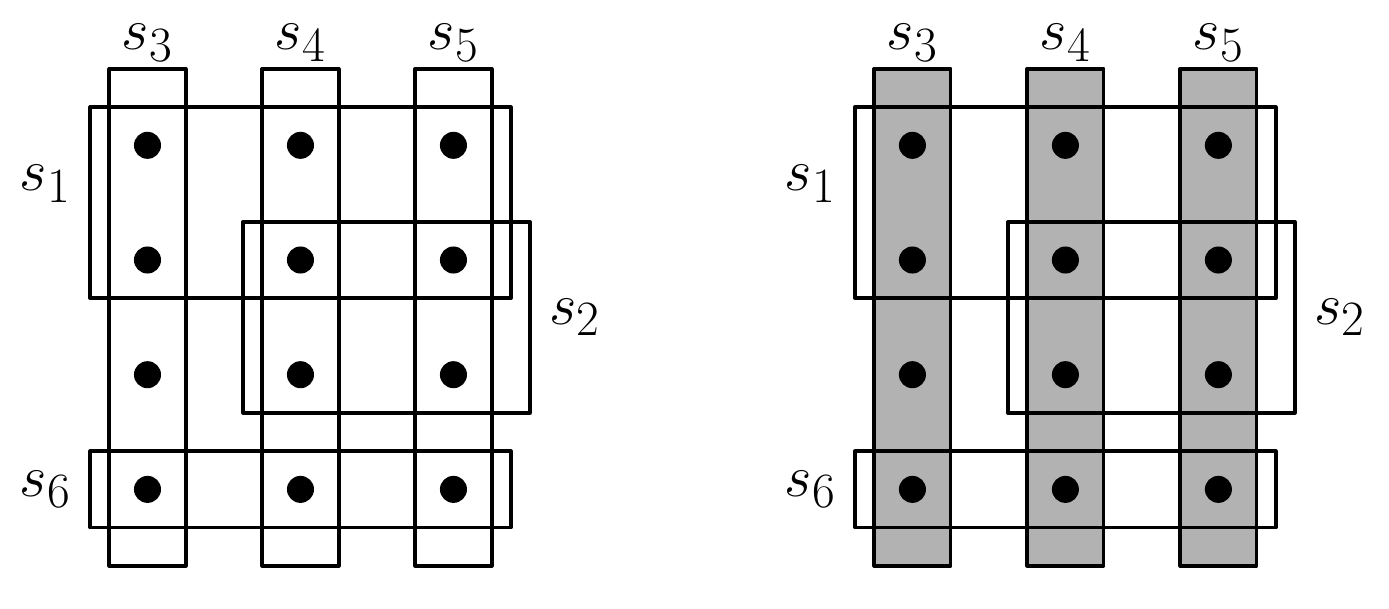
\includegraphics[width=0.65\linewidth]{figures/example}%
			\caption{Exemple d'instance du Set Cover Problem et solution optimale\cite{Mount2017}}%
			\label{fig:example}%
		\end{figure}
	\section{Complexité}
		\paragraph*{}
			Le SCP est un problème d'optimisation NP-difficile, et NP-complet dans sa forme décisionnelle. IL fait notamment parti des 21 problèmes NP-complets de \citeauthor{Karp1972}~\cite{Karp1972} et est NP-complet au sens fort \cite{garey2002computers}.
		\paragraph*{}
			La démonstration de la NP-complétude du problème a été réalisée par \citeauthor{Karp1972} en \citeyear{Karp1972} dans son article \citetitle{Karp1972}\cite{Karp1972}. Dans cet article, il réalise des réductions pour 21 problèmes réputés difficiles de combinatoire et de théorie des graphes comme représenté sur la figure \ref{fig:karp_reduction_tree}.
		\begin{figure}[H]
			\centering%
			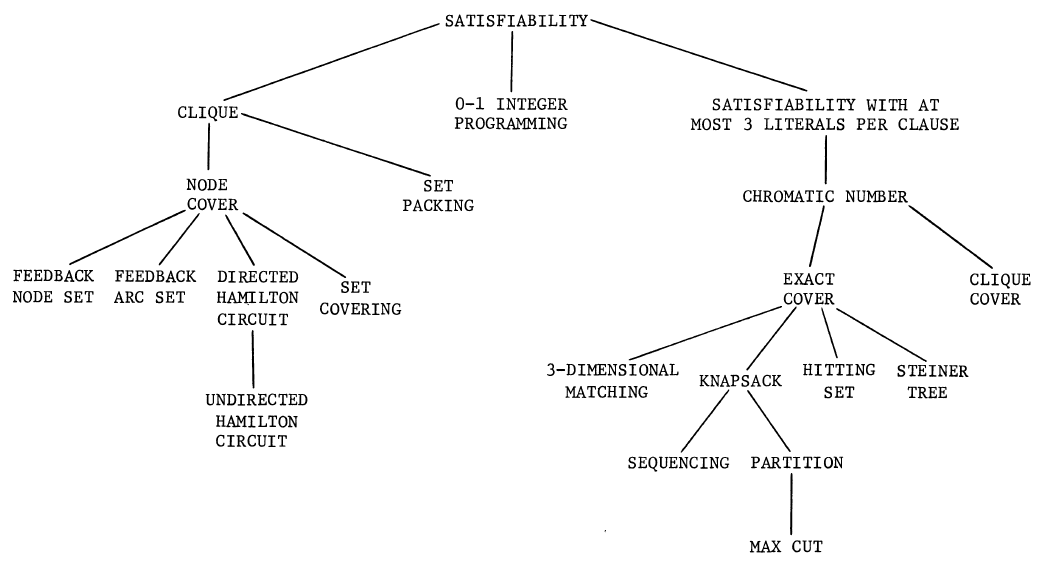
\includegraphics[width=\linewidth]{karp_reduction_tree}%
			\caption{Arbre des réductions réalisées par Karp\cite{Karp1972}}%
			\label{fig:karp_reduction_tree}%
		\end{figure}
		\paragraph*{}
			Concernant notre problème, \citeauthor{Karp1972} montre donc que le Boolean Satisfiability Problem (SATISFIABILITY) peut être réduit au Clique Problem (CLIQUE) qui peut etre réduit au Vertex/Node Cover Problem (NODE COVER) qui peut être réduit au Set Covering Problem (SET COVERING).
		\paragraph*{}
			Le théorème de Cook–Levin et sa démonstration publié en \citeyear{Cook1971} par \citeauthor{Cook1971} dans l'article \citetitle{Cook1971}\cite{Cook1971} prouve le Boolean Satisfiability Problem comme étant un problème NP-complet. Par réduction, le Set Covering Problem est donc aussi NP-complet.
		\paragraph*{}
			Pour ce qui est du Weighted Set Covering Problem (WSCP), c'est une généralisation du SCP et la réduction de ce dernier est évidente, il suffit de rajouter des poids tous égaux a une instance de SCP pour obtenir une instance de WSCP équivalente, le WSCP est donc lui aussi NP-complet.
	\section{État de l'art}
		\paragraph*{}
			Les algorithmes présentés dans cette section utilisent souvent le modèle de la relaxation lagrangienne.
			Cette relaxation consiste à supprimer des contraintes difficiles en les intégrant dans la fonction objectif en tant que pénalités.
			Les coefficients appliqués sont dans ce qu'on appelle le « vecteur multiplicateur de lagrange ».~\cite{fisher1985applications}
		\subsection{Méthodes exactes}
			\paragraph*{}
				La plupart des méthodes exactes les plus efficaces pour résoudre le problème de couverture d'ensemble sont
				des méthodes branch-and-bound
				dans lesquelles on calcule les bornes inférieures à l'aide d'une relaxation du problème en programmation
				linéaire.~\cite{caprara2000algorithms}
			\paragraph*{}
				\citeauthor{Beasley1987} a proposé un algorithme qui fonctionne de cette façon.
				Le nœud racine utilise la solution du programme linéaire relaxé, puis les bornes inférieures
				sont calculées à l'aide de la relaxation lagrangienne avec la descente de sous-gradient.~\cite{Beasley1987}
		\subsection{Méthodes approchées}
			\subsubsection{Méthodes voraces non optimales}\label{sec:soa-greedy}
				\paragraph*{}
					\citeauthor{Johnson:1973:AAC:800125.804034} a présenté dans son papier \citetitle{Johnson:1973:AAC:800125.804034}
					l'algorithme vorace standard pour le problème de couverture d'ensemble non pondéré.
					L'algorithme prend simplement le sous-ensemble qui couvre le plus
					d'éléments à chaque étape jusqu'à obtenir une solution valide. La complexité de l'algorithme est en \(O(mn)\) avec \(m\)
					le nombre d'éléments et \(n\) le nombre de sous-ensembles.~\cite{Johnson:1973:AAC:800125.804034}
					Cet algorithme n'est pas très efficace sur un problème de couverture d'ensemble pondéré car il n'en tient pas du
					tout compte.
				\paragraph*{}
					\citeauthor{Cormen:2009:IAT:1614191} ont présenté une version de l'algorithme utilisant une queue à priorité,
					permettant d'améliorer la vitesse de l'algorithme.~\cite{Cormen:2009:IAT:1614191}
				\paragraph*{}
					\citeauthor{Goldschmidt:1993:MGH:177276.177287} ont proposé une solution qui fonctionne en appliquant des
					combinaisons de plusieurs algorithmes. Des algorithmes approchés et exacts sont utilisés.
					La méthode exploite le fait qu'il est possible de trouver la solution optimale pour des ensembles de taille 2 au maximum
					en un temps polynomial. On exécute l'algorithme vorace standard de Johnson jusqu'à obtenir une taille maximale de 2 pour les
					ensembles, puis trouve la couverture optimale pour le reste, ce qui donne une solution améliorée.~\cite{Goldschmidt:1993:MGH:177276.177287}
			\subsubsection{Heuristiques}
				\paragraph*{}
					De nombreuses méthodes par heuristique sont basées sur l'observation que pour un vecteur multiplicateur de lagrange quasi-optimal
					le coût de lagrange donne une information fiable sur l'utilité générale de la sélection d'un sous-ensemble donné.
					De là, plutôt que d'utiliser les coûts originaux, on utilise les coûts de lagrange pour calculer les scores permettant
					de classer les différents sous-ensembles à sélectionner pour la solution optimale. Ces scores sont donnés
					à un algorithme vorace pour obtenir une solution valide.~\cite{caprara2000algorithms}
				\paragraph*{}
					\citeauthor{Beasley1990} a proposé un algorithme qui calcule à chaque itération de l'optimisation par sous-gradient une
					solution valide de la façon suivante : un ensemble \(S\) est initialisé avec les sous-ensembles sélectionnés
					par la solution de la relaxation lagrangienne. Puis, pour chaque point non couvert par \(S\),
					le sous ensemble avec le coût original le plus faible est ajouté à \(S\). Pour finir, les différents sous-ensembles
					de \(S\) sont considérés par ordre de coût original décroissant et on enlève le sous-ensemble \(j\) si \(S \backslash \{j\}\)
					est toujours une solution valide. À chaque itération on effectue un fixage de coût de lagrange pour réduire la taille
					du problème.~\cite{Beasley1990}	
				\paragraph*{}
					\citeauthor{jacobs1995lsh} ont proposée une approche basée sur le recuit simulé. Une solution initiale \(S\)
					est générée par un algorithme vorace qui à chaque itération sélectionne aléatoirement un point non couvert
					et ajoute à la solution le premier sous-ensemble qui couvre ce point. Après cette addition, les colonnes
					redondantes sont enlevées de la solution, et le processus est continué jusqu'à l'obtention d'une solution valide.
					Ensuite, on effectue un certain nombre d'itérations de recuit simulé : on choisi un sous-ensemble dans \(S\) aléatoirement
					et on l'enlève, puis on complète de manière vorace de manière à obtenir une autre solution valide \(S'\). Si \(S'\)
					est une meilleure solution que \(S\), \(S'\) remplace \(S\), sinon il remplace avec une certaine probabilitié qui
					décroit exponentiellement au fil des itérations.~\cite{jacobs1995lsh}
				\paragraph*{}
					\citeauthor{Brusco1999} ont ensuite proposé une amélioration à cette méthode.
					Premièrement, au lieu de choisir le sous-ensemble à enlever aléatoirement à chaque itération, on ne le fait plus
					que toutes les trois itérations. Pendant les deux itérations restantes, on choisi simplement le sous-ensemble qui
					laisse le moins de point non couvert possible. Deuxièmement, pour chaque sous-ensemble \(j\) de la solution,
					on utilise une liste de « morphs », qui sont tout simplement les autres sous-ensembles « similaires » à \(j\).
					Après avoir obtenu la solution partielle et tous les quatre sous-ennsemble ajouté pour la compléter, on itère
					sur tous les sous-ensembles de la solution partielle courante
					et on remplace chaque sous ensemble par l'un de ses « morphs » si cela améliore le ratio entre le coût actuel
					et le nombre de point couverts.~\cite{Brusco1999}
				\paragraph*{}
					\citeauthor{Afif1995} ont présenté une solution basée sur l'algorithme du flot de Ford-Fulkerson qui est un algorithme
					en temps polynomial.
					Il s'agit d'effectuer une transformation du problème en un graphe de flot à résoudre par une variante de l'algorithme
					de Ford-Fulkerson. Il est montré que le problème de couverture d'ensemble peut se réduire à un problème de flot minimal
					en temps polynomial.~\cite{Afif1995}
	\section{Représentation du problème}
		\subsection{Représentation mathématique}
			\paragraph*{}
				On reprend la notation:
				\begin{itemize}
					\item \(U = \{u_1, u_2, u_3, \dots, u_m\}\), ensemble univers composé de \(m\) points
					\item \(S = \{s_1, s_2, \dots, s_n\}\), famille de \(n\) sous-ensembles de \(U\)
				\end{itemize}
				et on pose \(M = \{1,\ldots,m\}\) et \(N = \{1,\ldots,n\}\).
			\paragraph*{Matrice d'incidence\\}
				On définit la matrice d'incidence \(A = \left(a_{i,j}\right)\) de taille \(m \times n\) avec
				\[\forall i \in M,\ \forall j \in N,\ a_{i,j} = \left\{
				    \begin{array}{ll}
				        1 & \text{si } u_i \in s_j \\
				        0 & \text{sinon}
				    \end{array}
				\right.\]
				\(a_{i,j} = 1\) signifiant donc que le point \(i\) est couvert par le sous-ensemble \(j\).
			\paragraph*{Vecteur coût\\}
				On définit le vecteur coût \(n\)-dimensionnel \(c = \left(c_j\right)\) avec \(\forall j \in N\), \(c_j\) le coût du sous ensemble \(j\).
			\paragraph*{Solution\\}
				On définit un vecteur solution comme un vecteur \(n\)-dimensionnel \(x = \left(x_j\right)\) avec
				\[\forall j \in N,\ x_j = \left\{
				    \begin{array}{ll}
				        1 & \text{si } u_i \text{ fait parti de la solution}\\
				        0 & \text{sinon}
				    \end{array}
				\right.\]
				La solution ayant comme coût \(\sum_{j \in N}{c_i x_i}\) et étant valide si
				\[\forall i \in M\ ,\sum_{j \in N}{a_{ij}x_i} \ge 1\]
		\subsection{Représentation dans notre projet}
			\paragraph*{}
				La première chose que l'on peut remarquer dans la représentation de notre problème, est que la matrice d'incidence \(A\) ainsi que le vecteur solution \(x\) ne contiennent que des valeurs booléennes (égales \(0\) ou \(1\)).
			\paragraph*{}
				La deuxième chose, qui est asse commune dans le champ de l'optimisation, et particulièrement vrai dans le cas des algorithmes que nous avons implémenté, est qu'une grande partie du temps de calcul est dédié a la vérification de la validité des solutions ainsi qu'a l'évaluation des solution par la fonction objectif.
			\paragraph*{}
				Notre fonction objective étant
				\[f(x) = \sum_{j \in N}{c_i x_i}\]
				Cette dernière peut être implémentée avec une boucle simple et sa complexité est en \(\mathcal{O}(n)\).
			\paragraph*{}
				Pour ce qui est de la vérification de la validité des solution, il faut s'assurer que:
				\[\forall i \in M\ ,\sum_{j \in N}{a_{ij}x_i} \ge 1\]
				Un algorithme évident est de faire deux boucles imbriquées, la première de longueur \(m\) sur les points et la deuxième de longueur \(n\) sur les sous-ensembles. Cet algorithme aurais alors une complexité en \(\mathcal{O}(mn)\). Une première optimisation serais d’arrêter la deuxième boucle au premier sous-ensemble qui couvre le point, cependant nous avons plutôt décider d'adopter une approche qui permet de prendre avantage des processeurs modernes (post-2013).
			\paragraph*{}
				En effet les processeurs modernes sont équipé d'instruction SIMD (Single Instruction Multiple Data), on peut notamment penser a l'AVX512 sur les processeurs Intel qui permet de réaliser des opérations sur 512 bits simultanément. Nous avons donc décider de stoker la matrice d'incidence \(A\) ainsi que le vecteur solution \(x\) sur les bits de types primitifs \Cpp{} afin de pouvoir leur appliquer des opérations simultanément. Nous allons considéré pour les paragraphes suivant un processeur 64 bits standard et le fait que les types primitifs courants sont sur 64 bits (ce qui est une simplification ne prenant pas en compte les possibles optimisations que le compilateur pourrais réaliser).
			\paragraph*{}
				Pour cela une classe \texttt{dynamic\_bitset}\cite{dynamicbitset}, implémentée par un membre du groupe, et permet d'utiliser un bitset dynamique (dont la taille n'est pas connue a la compilation) et d'appliquer toutes les opérations booléennes de façon optimisée en tirant avantage des instructions SIMD du processeur si elles sont présentes. De plus les processeur standards sont aussi équipés d'instructions pour connaitre le nombre de bits à \(1\) et la position du bit de poids le plus faible à \(1\), cela divisant donc la complexité du parcourt de \(x\) pour trouver le prochain sous-ensemble inclut dans la solution par jusqu’à 64. Et enfin le fait de stocker \(k\) information sur \(k\) bits au lieu de \(64k\), permet de faire une bien meilleur utilisation du cache processeur et nous permet de gagner énormément en performances.
			\paragraph*{}
				La matrice d'incidence \(A\) devient donc un vecteur de \(n\) bitsets de taille \(m\), un par sous-ensemble et le vecteur solution \(x\) devient un bitset de taille \(n\). La figure \ref{fig:representation_to_bitsets} illustre ce passage pour une instance a 5 points et 7 sous-ensembles.
			\begin{figure}[H]
				\centering%
				\resizebox{0.8\textwidth}{!}{\includestandalone{./figures/representation_to_bitsets}}%
				\caption{Passage de la représentation mathématique aux bitsets (instance a 5 points et 7 sous-ensembles)}%
				\label{fig:representation_to_bitsets}%
			\end{figure}
			\paragraph*{}
				Avec une telle représentation, la vérification de la validité d'une solution peut se faire efficacement en réalisant une opération booléenne \textit{OR} sur tout les bitsets \(S_i\) pour lesquels \(x_1\) est a \(1\) et en vérifiant que le bitset résultat de cette opération a tout ces bits a \(1\). La figure \ref{fig:solution_validity_check_function} représente cette opération.
			\begin{figure}[H]
				\centering%
				\resizebox{\textwidth}{!}{\includestandalone{./figures/solution_validity_check_function}}%
				\caption{Vérification de la validité d'une solution avec la représentation a base de bitsets (instance a 5 points et 7 sous-ensembles)}%
				\label{fig:solution_validity_check_function}%
			\end{figure}
			\paragraph*{}
				L'opération \textit{OR} sur les bitsets ainsi que la vérification que tout les bits sont a \(1\) est de complexité \(\mathcal{O}(1)\) pour un nombre de bits raisonnable (ce qui est largement le cas même pour les plus grandes instances que nous utiliserons). Notre algorithme de vérification de la validité d'une solution est donc en \(\mathcal{O}(n)\).
			\paragraph*{}
				La complexité des opérations sur notre problème étant donc toutes en \(\mathcal{O}(n)\), on ne s'occupera plus par la suite du nombre de points \(m\) et on dira qu'un problème avec \(m\) points et \(n\) sous-ensembles est un problème de taille \(n\).
	\section{Instances du problème}
		\subsection{OR-Library}
			\paragraph*{}
				On utilise les groupes d'instances mis a disposition par \citeauthor{OR-Library} dans son regroupement d'instances OR-Library\cite{OR-Library}. Parmis ces instances, celles de 4 à 6 proviennent l'article \citetitle{Balas1980}\cite{Balas1980} de \citeauthor{Balas1980}, celles de A à D proviennent de l'article \citetitle{Beasley1987}\cite{Beasley1987} de \citeauthor{Beasley1987} et celles de E à H proviennent de l'article \citetitle{Beasley1990}\cite{Beasley1990} de \citeauthor{Beasley1990}.
			\paragraph*{}
				Toutes les instances du problème de ces groupes on été générées en utilisant le shémas de \citeauthor{Balas1980}\cite{Balas1980} dans lequel le cout \(c_i\) de chaque colonne \(i\) est pris aléatoirement dans l'intervalle \(\llbracket0,100\rrbracket\), chaque colonne couvre au moins une ligne et chaque ligne est couverte par au moins deux clonnes.
			\paragraph*{}
			   Les propriétés de ces groupes d'instances sont décrites dans la table \ref{table:scp_problem_sets}, la densitée étant la proportion de \(1\) dans la matrice \(a_{i,j}\). La table \ref{table:orlibrary_scp_problems_optimal_solutions}, contient les valeure optimales pour les problèmes pour lesquels elle est connue.
			\begin{table}[H]
				\centering
				%!TEX root = ../set_cover_problem.tex
\begin{tabular}{*{5}{C{65pt}}}
	\toprule
	Groupe d'instances & Nombre de lignes (\(m\)) [points] & Nombre de colonnes (\(n\)) [sous-ensembles] & densité (\%) & Nombre d'instances du groupe\\
	\midrule
	4 & 200 & 1000 & 2 & 10\\
	5 & 200 & 2000 & 2 & 10\\
	6 & 200 & 1000 & 5 & 5\\
	A & 300 & 3000 & 2 & 5\\
	B & 300 & 3000 & 5 & 5\\
	C & 400 & 4000 & 2 & 5\\
	D & 400 & 4000 & 5 & 5\\
	E & 500 & 5000 & 10 & 5\\
	F & 500 & 5000 & 20 & 5\\
	G & 1000 & 10000 & 2 & 5\\
	H & 1000 & 10000 & 5 & 5\\
	\bottomrule
\end{tabular}
				\caption{Groupes d'instances du SCP utilisées\cite{OR-Library,Balas1980,Beasley1987,Beasley1990}}
				\label{table:scp_problem_sets}
			\end{table}
			\begin{table}[H]
				\centering
				\begin{minipage}[t]{0.45\linewidth}
					\centering
					%!TEX root = ../set_cover_problem.tex
\begin{tabular}{*{2}{C{65pt}}}
	\toprule
	Problem number & Optimal solution value\\
	\midrule
	4.1 & 429\\
	4.2 & 512\\
	4.3 & 516\\
	4.4 & 494\\
	4.5 & 512\\
	4.6 & 560\\
	4.7 & 430\\
	4.8 & 792\\
	4.9 & 641\\
	4.10 & 514\\
	\midrule
	5.1 & 253\\
	5.2 & 302\\
	5.3 & 226\\
	5.4 & 242\\
	5.5 & 211\\
	5.6 & 213\\
	5.7 & 293\\
	5.8 & 288\\
	5.9 & 279\\
	5.10 & 265\\
	\bottomrule
\end{tabular}
				\end{minipage}
				\begin{minipage}[t]{0.45\linewidth}
					\centering
					%!TEX root = ../set_cover_problem.tex
\begin{tabular}{*{2}{C{65pt}}}
	\toprule
	Problem number & Optimal solution value\\
	\midrule
	A.1 & 253\\
	A.2 & 252\\
	A.3 & 232\\
	A.4 & 234\\
	A.5 & 236\\
	\midrule
	B.1 & 69\\
	B.2 & 76\\
	B.3 & 80\\
	B.4 & 79\\
	B.5 & 72\\
	\midrule
	C.1 & 227\\
	C.2 & 219\\
	C.3 & 243\\
	C.4 & 219\\
	C.5 & 215\\
	\midrule
	D.1 & 60\\
	D.2 & 66\\
	D.3 & 72\\
	D.4 & 62\\
	D.5 & 61\\
	\bottomrule
\end{tabular}
				\end{minipage}
				\caption{Solutions optimales des instances du SCP utilisée\cite{Beasley1990}}
				\label{table:orlibrary_scp_problems_optimal_solutions}
			\end{table}
		\subsection{Instances générées}
			\paragraph*{}
				Les instances de OR-Library étant de grande taille, elles ne nous permettent pas de tester nos méthodes exactes, nous avons donc codé un générateur d'instances utilisant la même méthode qu'utilisée pour celles de OR-Library (shémas de \citeauthor{Balas1980}\cite{Balas1980}).
			\paragraph*{}
				Afin de benchmarcker les différentes méthodes implémentées, notamment les méthodes exactes avec des instances identiques pour avoir des valeures comparables, nous avons utilisé le générateur pour réaliser un ensemble d'instances de test de taille \(2\) a \(100\) avec \(200\) points.
			\paragraph*{}
				La table \ref{table:generated_scp_problems_optimal_solutions} regroupe les solutions optimales de nos instances lorsque les méthodes exactes nous ont permis de les obtenir.
			\paragraph*{}
			\begin{table}[H]
				\centering
				\begin{minipage}[t]{0.3\linewidth}
					\centering
					%!TEX root = ../set_cover_problem.tex
\begin{tabular}{*{2}{C{65pt}}}
	\toprule
	Problem size & Optimal solution value\\
	\midrule
	2 & 65\\
	3 & 63\\
	4 & 165\\
	5 & 183\\
	6 & 220\\
	7 & 224\\
	8 & 230\\
	9 & 163\\
	10 & 287\\
	11 & 253\\
	12 & 223\\
	13 & 345\\
	14 & 336\\
	15 & 391\\
	16 & 356\\
	17 & 249\\
	18 & 243\\
	19 & 264\\
	20 & 288\\
	21 & 390\\
	22 & 300\\
	23 & 234\\
	24 & 244\\
	25 & 274\\
	26 & 460\\
	27 & 336\\
	28 & 315\\
	29 & 253\\
	30 & 256\\
	31 & 327\\
	32 & 409\\
	33 & 401\\
	34 & 334\\
	\bottomrule
\end{tabular}
				\end{minipage}
				\begin{minipage}[t]{0.3\linewidth}
					\centering
					%!TEX root = ../set_cover_problem.tex
\begin{tabular}{*{2}{C{65pt}}}
	\toprule
	Problem size & Optimal solution value\\
	\midrule
	35 & 185\\
	36 & 411\\
	37 & 310\\
	38 & 247\\
	39 & 247\\
	40 & 358\\
	41 & 398\\
	42 & 368\\
	43 & 507\\
	44 & 360\\
	45 & 305\\
	46 & 263\\
	47 & 278\\
	48 & 214\\
	49 & 270\\
	50 & -\\
	51 & 317\\
	52 & 185\\
	53 & 275\\
	54 & 261\\
	55 & 302\\
	56 & 261\\
	57 & 279\\
	58 & -\\
	59 & -\\
	60 & 309\\
	61 & 129\\
	62 & 260\\
	63 & -\\
	64 & 290\\
	65 & 200\\
	66 & -\\
	67 & 195\\
	\bottomrule
\end{tabular}
				\end{minipage}
				\begin{minipage}[t]{0.3\linewidth}
					\centering
					%!TEX root = ../set_cover_problem.tex
\begin{tabular}{*{2}{C{65pt}}}
	\toprule
	Problem size & Optimal solution value\\
	\midrule
	68 & 231\\
	69 & -\\
	70 & 225\\
	71 & -\\
	72 & -\\
	73 & 141\\
	74 & -\\
	75 & -\\
	76 & -\\
	77 & 226\\
	78 & 186\\
	79 & 166\\
	80 & 276\\
	81 & -\\
	82 & -\\
	83 & -\\
	84 & -\\
	85 & -\\
	86 & -\\
	87 & -\\
	88 & -\\
	89 & 219\\
	90 & -\\
	91 & -\\
	92 & -\\
	93 & -\\
	94 & -\\
	95 & -\\
	96 & -\\
	97 & -\\
	98 & -\\
	99 & -\\
	100 & -\\
	\bottomrule
\end{tabular}
				\end{minipage}
				\caption{Solutions optimales des instances générées}
				\label{table:generated_scp_problems_optimal_solutions}
			\end{table}
	\section{Méthodes exactes}
		\subsection{Recherche exhaustive}
			\paragraph*{}
				La méthode exacte la plus simple est encore la recherche exhaustive, dans notre cas, cela consiste a tester toutes les valeurs possibles du vecteur de solution \(x\). Ce vecteur étant un vecteur booléen, il y a \(2^n\) possibilité pour un vecteur de taille \(n\) qui correspond a un problème de taille \(n\).
			\paragraph*{}
				Pour le SCP simple, il n'est pas nécessaire de tester toutes les permutations possibles, il suffit de commencer par les permutations de 1 bit, puis 2,3\ldots et dès que la permutation est une solution valide, cette dernière est la solution optimale puisque la première valide en le moins de sous-ensembles possibles.
			\paragraph*{}
				Nous avons commencé par utiliser les algorithmes classiques connu qui sont récursifs, mais ces derniers atteignent très rapidement la limite de stack du programme de par le nombre élevé d'appels récursifs pour les taille de bitset dont nous avons besoin. Ils ne sont donc pas envisageables pour notre problème.
			\paragraph*{}
				Nous avons donc réalisé un générateur de permutations G1 qui utilise une méthode s'inspirant de la programmation dynamique. En effet les permutations de \(k\) bits parmi \(n\) sont les permutations de \(k\) bits parmi \(n-1\) avec le \(n\)-ème bit a \(0\) ajouté aux permutations de \(k-1\) bits parmi \(n-1\) avec le \(n\)-ème bit a \(1\). En notant \(P_k^n\) les permutations de \(k\) bits parmi \(n\), on peut donc généré facilement \(P_k^n\) a l'aide de \(P_k^{n-1}\) et de \(P_{k-1}^{n-1}\).
			\paragraph*{}
				Le générateur G1 génère donc les \(P_i^n\) pour \(i \in \llbracket 0, n \rrbracket\) en générant successivement les \(P_i^t\) pour \(t\in \llbracket 1, n \rrbracket\) en utilisant les \(P_i^t\) de la génération précédente comme représenté sur la figure \ref{fig:g1_permutations}.
			\begin{figure}[H]
				\centering%
				\resizebox{0.4\textwidth}{!}{\includestandalone{./figures/g1_permutations}}%
				\caption{Méthode de génération des \(\forall i \in \llbracket 0, n \rrbracket,\ P_i^n\) du générateur G1}%
				\label{fig:g1_permutations}%
			\end{figure}
			\paragraph*{}
				Le problème avec générateur G1 est qu'il a besoin de stocker toutes les permutations de la génération précédente pour générer la suivante or le nombre de permutation augmente en \(2^n\) et son utilisation de RAM pour stocker les permutations dépasse les 8Go pour générer les permutations sur un bitset de taille 27 (voir figure \ref{figure:permutations_generators_ram}).
			\begin{figure}[H]
				\centering
				%!TEX root = ../set_cover_problem.tex
\begin{tikzpicture}
	\begin{axis}[
		width=\linewidth,
		height=0.5\linewidth,
		xlabel={bitset size (bits number)},
		ylabel={ram usage (Go)},
		xmin=0, xmax=40,
		ymin=0, ymax=9,
		legend style={
			cells={
				anchor=west
			},
			legend pos=north west,
		},
	]
		\addplot[smooth,color=blue,mark=*] table{plots/g1_ram.data};
		\addlegendentry{G1: ram expensive generator}
		\addplot[smooth,color=red,mark=*] table{plots/g2_ram.data};
		\addlegendentry{G2: cpu expensive generator}
		\addplot[smooth,color=cyan,mark=*] table{plots/g3_ram.data};
		\addlegendentry{G3: counter generator}
	\end{axis}
\end{tikzpicture}%%
				\caption{Utilisation de la RAM par les générateurs de permutations}
				\label{figure:permutations_generators_ram}
			\end{figure}
			\paragraph*{}
				Nous avons donc réalisé un générateur G2 qui ne nécessite pas de stocker les permutation des génération précédentes mais va les construires dynamiquement au fil de la génération des \(P_i^n\), ce générateur est donc bien moins performant (voir figure \ref{figure:plots/permutations_generators_time}) mais a l'avantage de ne pas consommer excessivement de RAM (voir figure \ref{figure:permutations_generators_ram}). Le générateur G2 peut générer les \(P_i^n\) jusqu'à \(n = 32\) en moins d'une heure, ce qui est bien loin d’être suffisant pour des grandes instances tels que celles de OR-Library.
			\paragraph*{}
				Les générateurs G1 et G2 génèrent les permutations de 1 bit, puis 2,3\ldots afin d’être efficace pour le SCP simple mais il est possible de générer ces permutations de façon plus efficace si on ne restrein pas l'ordre de génération. Nous avons donc codé un générateur G3 WSCP qui est plus performant que G1 et G2 mais ne garanti pas un ordre croissant sur le nombre de bits a \(1\). G3 est donc moins performant que G1 et G2 pour le SCP mais plus performant pour le WSCP.
			\paragraph*{}
				Le générateur G3 génère les permutations en considérant le bitset comme la représentation binaire d'un nombre, il suffit de commencer a 0 et d'incrémenter le nombre représenté jusqu'à retourner a 0 pour être passé par toutes les valeurs représentables sur \(n\) bits et donc toutes les permutations. L'algorithme consiste donc à appliquer donc successivement l'algorithme d'incrément binaire qui commence par le bit de poids le plus faible et remonte les bits en transformant les \(1\) en \(0\) jusqu’à arriver a la fin du bitset ou a un \(0\) qu'il transforme en \(1\).
			\paragraph*{}
				Les 3 générateurs réalisent (en pire cas pour G3) \(\mathcal{O}(n)\) opération pour générer chaque permutation, la complexité des 3 générateurs pour générer les \(2^n\) permutations est donc en \(\mathcal{O}(n2^n)\). Pour les comparer, on réalise donc une étude empirique dont les résultats sont visibles sur les graphiques de la figure \ref{figure:plots/permutations_generators_time}. Comme prévu, le générateur G3 est le plus performant, cependant il n'est pas adapté pour le SCP simple.
			\begin{figure}[H]
				\centering
				%!TEX root = ../set_cover_problem.tex
\begin{tikzpicture}
	\begin{axis}[
		width=\linewidth,
		height=0.6\linewidth,
		xlabel={taille du bitset (nombre de bits)},
		ylabel={temps (s)},
		xmin=0, xmax=40,
		ymin=0, ymax=2500,
		legend style={
			cells={
				anchor=west
			},
			legend pos=north west,
		},
	]
		\addplot[smooth,color=blue,mark=square*] table{plots/g1_time.data};
		\addlegendentry{G1: ram expensive generator}
		\addplot[smooth,color=red,mark=*] table{plots/g2_time.data};
		\addlegendentry{G2: cpu expensive generator}
		% \addplot[
		% 	green,
		% 	domain=0:33,
		% 	samples=330,
		% ]{1.556624216*10^(-7) * e^(7.298880681*10^(-1)*x)};
		% \addlegendentry{\(1.556624216.10^{-7}e^{7.298880681.10^{-1}x}\)}
		\addplot[smooth,color=cyan,mark=triangle*] table{plots/g3_time.data};
		\addlegendentry{G3: counter generator}
		\addplot[
			green,
			domain=0:40,
			samples=400,
		]{4.114961289*10^(-9) * (e^(0.693072216*x) + 1};
		\addlegendentry{\(4.114961289.10^{-9}\left(e^{0.693072216x} + 1\right)\)}
	\end{axis}
\end{tikzpicture}%\\
				%!TEX root = ../set_cover_problem.tex
\begin{tikzpicture}
	\begin{semilogyaxis}[
		width=\linewidth,
		height=0.6\linewidth,
		xlabel={bitset size (bits number)},
		ylabel={time (s) [échelle logarithmique]},
		xmin=0, xmax=40,
		ymin=0, ymax=10000,
		legend style={
			cells={
				anchor=west
			},
			legend pos=north west,
		},
	]
		\addplot[smooth,color=blue,mark=*] table{plots/g1_time.data};
		\addlegendentry{G1: ram expensive generator}
		\addplot[smooth,color=red,mark=*] table{plots/g2_time.data};
		\addlegendentry{G2: cpu expensive generator}
		% \addplot[
		% 	green,
		% 	domain=0:33,
		% 	samples=330,
		% ]{1.556624216*10^(-7) * e^(7.298880681*10^(-1)*x)};
		% \addlegendentry{\(1.556624216.10^{-7}e^{7.298880681.10^{-1}x}\)}
		\addplot[smooth,color=cyan,mark=*] table{plots/g3_time.data};
		\addlegendentry{G3: counter generator}
		\addplot[
			green,
			domain=0:40,
			samples=400,
		]{4.114961289*10^(-9) * (e^(0.693072216*x) + 1};
		\addlegendentry{\(4.114961289.10^{-9}\left(e^{0.693072216x} + 1\right)\)}
	\end{semilogyaxis}
\end{tikzpicture}%%
				\caption{Temps nécessaire pour générer toutes les permutations d'un bitset}
				\label{figure:plots/permutations_generators_time}
			\end{figure}
			\paragraph*{}
				En se fiant aux données de notre étude, sur l'ordinateur de test, la durée nécessaire au générateur G3 pour générer les permutations d'un vecteur de taille \(x\) est approximable par la fonction \(4.114961289.10^{-9}\left(e^{0.693072216x} + 1\right)\). Si l'on voulait résoudre les plus petites instances de OR-Library à \(1000\) éléments, il faudrait donc un temps théorique de \(4 \times 10^{492}\)s au générateur G3 pour générer les permutations du vecteur \(x\) et tester toutes les possibilités. Au vu de inefficacité de la recherche exhaustive nous avon décidé d'implémenté une seconde méthode exacte: le branch and bound.
		\subsection{Branch and bound}
			\paragraph*{}
				TODO
			\begin{figure}[H]
				\centering
				%!TEX root = ../set_cover_problem.tex
\begin{tikzpicture}
	\begin{axis}[
		width=\linewidth,
		height=0.5\linewidth,
		xlabel={bitset size (bits number)},
		ylabel={ram usage (Go)},
		xmin=0, xmax=40,
		ymin=0, ymax=9,
		legend style={
			cells={
				anchor=west
			},
			legend pos=north west,
		},
	]
		\addplot[smooth,color=blue,mark=*] table{plots/g1_ram.data};
		\addlegendentry{G1: ram expensive generator}
		\addplot[smooth,color=red,mark=*] table{plots/g2_ram.data};
		\addlegendentry{G2: cpu expensive generator}
		\addplot[smooth,color=cyan,mark=*] table{plots/g3_ram.data};
		\addlegendentry{G3: counter generator}
	\end{axis}
\end{tikzpicture}%%
				\caption{Utilisation de la RAM par les générateurs de permutations}
				\label{figure:permutations_generators_ram}
			\end{figure}
		\paragraph*{}
			Il existe une méthode exacte plus efficace qui utilise la méthode Branch and Bound ainsi que le Simplexe (pour résoudre une version
			du problème linéaire relaxée)~\cite{caprara2000algorithms}.
	\section{Méthodes approchées}
		\subsection{Algorithmes voraces}
			\paragraph*{}
				Nous avons commencé par implémenter des algorithmes voraces qui permettent de trouver des solutions approchées très rapidement.
			\paragraph*{}
				Le premier algorithme que nous avons implémenté est celui de
				\citeauthor{Johnson:1973:AAC:800125.804034}~\cite{Johnson:1973:AAC:800125.804034} présenté dans la section~\ref{sec:soa-greedy}
				où l'on intègre dans la solution les sous-ensembles couvrant le plus de point d'abord.
				On utilise le nombre de points qu'un sous-ensemble permet de couvrir de façon non redondante comme score.
			\paragraph*{}
				Pour le problème \emph{A.1} dont la solution optimale est \(253\), on obtient la solution de coût \(1444\) suivante :
			\begin{lstlisting}
[info] found unweighted greedy solution with 42 subsets cost of 1444 in 0.108285s
[info] Unweighted greedy solution: scp::Solution{
	selected subsets number = 42,
	selected subsets = 7, 32, 112, 132, 134, 136, 188, 191, 244, 245, 248, 274, 299, 392, 399, 428, 548, 816, 819, 922, 925, 960, 1042, 1068, 1096, 1161, 1208, 1271, 1300, 1302, 1412, 1418, 1454, 1505, 1565, 1971, 2056, 2154, 2341, 2462, 2752, 2941,
	cover all points = true,
	cost = 1444,
}\end{lstlisting}
			\paragraph*{}
				Pour un problème de couverture d'ensembles pondéré, cet algorithme est très mauvais.
				Nous avons donc décidé d'implémenter une version de l'algorithme qui prend en compte le coût des sous ensembles pour
				sélectionner lequel ajouter.
				Pour cela, nous utilisons le rapport \(\frac{n}{c}\) avec \(n\) le nombre de points actuellement non couverts que le
				sous-ensemble nous permettrait de couvrir et \(c\) le coût du sous-ensemble. C'est à dire le rapport de l'utilité sur
				le coût de la même façon que présenté dans le cours dans le chapitre sur les algorithmes voraces.
			\paragraph*{}
				De la même façon que précédememnt, pour le problème \emph{A.1} dont la solution optimale est \(253\), on obtient cette fois
				une solution de coût \(288\) :
			\begin{lstlisting}
[info] found weighted greedy solution with 89 subsets and cost of 288 in 0.564261s
[info] Weighted greedy solution: scp::Solution{
	selected subsets number = 89,
	selected subsets = 0, 1, 2, 3, 4, 5, 6, 7, 8, 9, 10, 11, 12, 13, 14, 15, 16, 17, 18, 19, 20, 21, 22, 23, 25, 27, 28, 30, 32, 33, 34, 37, 38, 39, 40, 42, 45, 46, 47, 48, 49, 50, 51, 54, 55, 59, 62, 63, 65, 66, 67, 69, 74, 76, 77, 78, 85, 86, 87, 88, 89, 90, 91, 92, 94, 97, 104, 105, 108, 112, 114, 115, 116, 117, 122, 123, 132, 137, 143, 162, 164, 172, 188, 189, 191, 214, 221, 268, 331,
	cover all points = true,
	cost = 288,
}\end{lstlisting}
			\paragraph*{}
				Utiliser le ratio utilité / coût nous permet donc d'obtenir une solution bien meilleure. On constate que dans le cas du
				problème de couverture d'ensemble pondéré, la meilleure solution n'est pas toujours celle qui utilise le moins de
				sous-ensembles. En effet, cette dernière solution utilise \(89\) solutions contre \(42\).
		\subsection{Méta-heuristiques}
			\subsubsection{Recuit simulé}
				TODO
			\subsubsection{Algorithme génétique}
				TODO
	\section{Conclusion}
		\paragraph*{}
			En tant que problème NP complet, la méthode exacte avec le branch-and-bound peut être très rapide ou très lent selon la configuration du problème.
			Pour résoudre des problèmes de taille supérieure, il nous a fallu implémenter des méthodes approchées.
			TODO
	\newpage\printbibliography[heading=bibintoc]{}
\end{document}

% Problem set        Files
% 4                  scp41, ..., scp410
% 5                  scp51, ..., scp510
% 6                  scp61, ..., scp65
% A                  scpa1, ..., scpa5
% B                  scpb1, ..., scpb5
% C                  scpc1, ..., scpc5
% D                  scpd1, ..., scpd5
% E                  scpe1, ..., scpe5

% Problem set        Files
% E                  scpnre1, ..., scpnre5
% F                  scpnrf1, ..., scpnrf5
% G                  scpnrg1, ..., scpnrg5
% H                  scpnrh1, ..., scpnrh5
